\documentclass[times, utf8, zavrsni]{fer}
\usepackage{booktabs}
\usepackage{indentfirst}

\begin{document}

% TODO: Navedite broj rada.
\thesisnumber{4350}

% TODO: Navedite naslov rada.
\title{Razvoj podatkovnog sloja i aplikacijske logike za potrebe sustava elektroničkog učenja}

% TODO: Navedite vaše ime i prezime.
\author{Alen Murtić}

\maketitle

% Ispis stranice s napomenom o umetanju izvornika rada. Uklonite naredbu \izvornik ako želite izbaciti tu stranicu.
\izvornik

% Dodavanje zahvale ili prazne stranice. Ako ne želite dodati zahvalu, naredbu ostavite radi prazne stranice.
\zahvala{}

\tableofcontents

\chapter{Uvod}
Znanje i prenošenje znanja najznačajniji je faktor sve bržeg razvoja ljudske civilizacije, iako je često nailazilo na prepreke u širenju. Prije početka 20. stoljeća ponajveći je problem bila dostupnost znanja, a ta je prepreka postajala sve manja izumima kao što su tiskarski stroj, sveučilište te obveznim školstvom i masovnom proizvodnjom knjiga. Dostupnog znanja danas je minoran ili čak nepostojeći problem, no to je stvorilo novi izazov - odabir pravog načina učenja. Moderno elektroničko doba samo ga je još pojačalo jer je ogromna količina e-knjiga od korisnika udaljena na samo nekoliko klikova.
\par
Moderni svijet donosi golemu količinu dostupnih informacija što je dovelo do toga da je ljudska pažnja sve neodređenija, a vrijeme fokusa sve kraće. Moderne generacije nemaju imperativ učenja kao njihovi preci, uglavnom zato što nikada nisu iskusile težinu ne-modernog života. Stoga se može dogoditi da čovjek željan znanja jednostavno odustane zbog ogromne količine mogućnosti, a posebno zbog činjenice se samo u ponekim školskim sustavima uči kako učiti.
\par
Shvativši da je znanje i prenošenje znanja izuzetno bitno te da je moderni svijet stvorio nove izazove učenju, postavlja se pitanje kako poboljšati njegovu kvalitetu? Odgovor je relativno jednostavan: pretvoriti učenje u nešto zanimljivo i jednostavno za korištenje, ali ipak izazovno i korisno - specijalizirane aplikacije, tj. sustave za elektroničko učenje.
\par
Ovaj završni rad opisat će što su sustavi za elektroničko učenje, što znači da je takav sustav inteligentan, neke od algoritama inteligencije, kako trebaju izgledati podatkovni i aplikacijski slojevi takvog sustava te objasniti što su oni uopće. U konačnici, temeljem principa navedenih u teoretskom dijelu, opisat će podatkovni i aplikacijski sloj sustava koji sam implementirao.


\chapter{Sustavi za elektroničko učenje}
Ideja sustava za elektroničko učenje je ujediniti postupak prenošenja informacija, upijanja novih činjenica i provjere znanja, baš kao na akademskim institucijama. No, prednosti sustava za elektroničko učenje nad tradicionalnim akademskim institucijama su veća prostorna dostupnost (praktički jedini uvjet sudjelovanja je internetska povezanost) te brže ažuriranje gradiva novim informacijama u odnosu na spori obrazovni sustav.
\par
Sustavi za elektroničko učenje mogu biti dio nekog formalnog obrazovnog sustava ili samostalni. Moodle je primjer sustava za elektroničko učenje čiji je cilj obavljati samo dio obrazovanja, uglavnom provjere znanja i prenošenja informacija (materijala za učenje). Od korisnika se očekuje da sam proučava te materijale ili pohađa predavanja predmeta unesenog na sustav Moodle. Samostalni sustavi za elektroničko učenje trebali bi imati dostupne sve elemente učenja jer samo tako mogu osigurati kvalitetu. Eventualno može nedostajati formalna provjera znanja ako je sustav dizajniran tako da je postupak upijanja novih činjenica rigorozan u korištenju da ga korisnik ni u kojem slučaju ne može preskočiti ili ignorirati. 
\par
Neki od popularnih i besplatnih sustava za elektroničko učenje su Codeacademy, Doulingo i Coursera. Coursera je zanimljiv koncept učenja koji na internet stranicu prenosi predmete stvarnih sveučilišta. Ona je za kranjeg korisnika samostalna, no stvaranje njezinog sadržaja nije. Duolingo Najpoznatiji akamdemski sustav za učenje je Moodle, a na FER-u se također koriste Ahyco i Ferko.
\par
Ahyco, Ferko
\pagebreak
\section{Inteligentni sustavi za elektroničko učenje (ITS)}
Inteligentni sustavi za elektroničko učenje posebna su vrsta sustava za elektroničko učenje koja korisniku pruža reakcije ili upute prilagođene isključivo njemu. Cilj svakog ITS je smanjiti ovisnost korisnika sustava o ljudskim učiteljima. Za razliku od ljudi, elektronički sustavi se ne umaraju, ne stare, gotovo uvijek imaju vremena za učenika. Naravno, inteligentni sustavi za elektroničko učenje također imaju svoje limite: kvalitetni su koliko je kvalitetan dizajner sustava, ne mogu pratiti fizičke reakcije korisnika i iskustveno zaključivati iz njih te, ipak, ne mogu biti potpuno individualni jer bi u tom slučaju količina praćenih podataka morala biti enormna. 

\subsection{Povijest ITS-a i zaključci iz nje}

\subsubsection{Mehanički strojevi za učenje}
Ideja inteligentnih sustava za učenje nije nastala tek u 21. stoljeću, dapače, već u 17. st. dvojica od najvećih europskih matematičara, Blaise Pascal i Gottfried Wilhelm Leibniz razmatrali su koncepte zaključivanja uz pomoć strojeva. Pravi zamah elektroničko učenje dobiva u 20.
\par
Prvi značajan korak prema učenju uz pomoć strojeva je napravio Sidney Leavitt Presley, profesor na Sveučilištu Ohio, koji je izumio stroj za samoocjenjivanje. Korisnik je odgovarao na pitanja s višestrukim izborom, stroj bi spremao odgovore te na kraju seta pitanja dao povratnu poruku o točnosti odgovora. Taj pristup koristi se i danas u većini akademskih sustava za ocjenivanje, sva tri, Moodle, Ferko i Ahyco ga koriste.

\begin{figure}[htb]
	\centering
	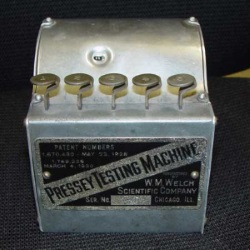
\includegraphics[]{img/pressey.jpg}
	\caption{Stroj za ocjenjivanje S. L. Presleyja}
	\label{fig:pressey}
\end{figure}

Iako su mehanički strojevi pružili kvalitetan početak ideje, jasno je da zbog neefleksibilnosti i skupoće izrade nikada nisu mogli prijeći fazu demonstracije. No, računalne aplikacije je lako umnožavati i mijenjati. Zato su one pogodne za razvoj sustava za učenje, ovog puta elektroničkih.

\subsubsection{Početak elektroničkih sustava za učenje}
U ranim godinama razvoja računala i računarstva napravljeni su mnogi koncepti bliskih tematika, npr. Turingov test, ideja umjetne inteligencije i strojnog učenja, no sustavi za učenje kao koncept kakav danas postoji je relativno zanemaren. Jedini važan napredak su definiranja gramatika u računarstvu, kao jednog od budućih načina parsiranja korisnikovih odgovora. No, dolaskom računala u širu upotrebu, u američkim školama se stvaraju CAI (\textit{Computer-Assisted instruction}) projekti s ciljem učenja programiranja. CAI sustav je takav da se korisniku prezentira neki materijal s uputom korištenja, nakon čega on na \textit{input-output} principu komunicira s računalom. Najbolji primjer nečega sličnog CAI sustavu u današnje vrijeme je Codeacademy. U početku se CAI koristio u učionicama, a ne individualno, ali na sličnom principu korištenja.

\begin{figure}[htb]
	\centering
	\includegraphics[]{img/CAI_shema.jpg}
	\caption{Shema rada pomoću CAI sustava}
	\label{fig:cai}
\end{figure}

\par
Velik korak za stvaranje ITS-a napravio je Jaime Carbonell koji je 1970. postavio tezu da "sustavi za učenje ne moraju biti samo alat, nego i učitelj". U 1970.-ima je najpopularnije novo područje bila umjetna inteligencija temeljena na znanju. Najpoznatiji primjer takvog sustava je \textit{Dendral}, sustav zaključivanja o kemijskim strukturama korištenim u organskoj kemiji. Izgradnja složenijih sustava je bila lakša zbog poboljšanja brzine računala što je fokus rada konačno maknulo s tehnologije na tehniku. 
\par
Početkom 1980. umjetna inteligencija se pomiče k neuronskim mrežama i kognitivnoj psihologiji što otvara prostor razvoju sustava za elektroničko učenje zbog sličnih područja interesa. To dovodi do stvaranja koncepta ICAI-ja (\textit{Intelligent Computer Assisted Instruction}), vrste CAI sustava koji bi radio na principu prilagođenog posluživanja instrukcija. ICAI je jako blizu modernom konceptu ITS-a, jedina razlika između njih je što ICAI ne pokušava modelirati znanje korisnika.

\subsubsection{ITS u doba interneta i analize podataka}
Najvažniji korak za veću primjenu elektroničkog učenja je početak masovnog korištenja interneta. Internet je konačno omogućio neovisnost fizičkih pozicija korisnika sustava i kvalitete znanja koju mu sustav može pružiti. Slabost prijašnjih rješenja je bila u neadekvatnoj aktualizaciji sustava zbog činjenice da su se morali distribuirati na prijenosnim medijima. Nije slučajno da su svi sustavi koje sam na početku nabrojao internetske stranice.
\par  TODO nekakva slika internet connecting world
\par
Analiza podataka, \textit{data mining}, \textit{big data} i \textit{data science} je najveći korak u razvoju inteligencije ITS-a. Iako su principi analize podataka bili matematički postavljeni i prije 1990.-ih, rastom brzine računala, popularizacijom SQL-a i internet tražilica, analiza podataka doživjela je pravi \textit{boom} zadnjih 20-tak godina. Razlog tolike važnosti analize podataka u inteligenciji ITS-a je što kompleksnost procesa učenja (čime se bavi kognitivna psihologija), "udaljnost" sustava i potreba za prilagođenim (personaliziranim) sadržajem korisniku. Ti faktori se jednostavno ne mogu opisati malim brojem varijabli. Svaki učitelj kroz godine upoznaje nove učenike te nadopunjuje svoje znanje i tehniku, baš kao što bi ITS bio spreman za nadogradnju temeljem iskustva korištenja.
\par
Za razliku od UI čije rezultate velike tvrtke sigurno mogu naplatiti, razvoj sustava za inteligentno učenje je donedavno bio guran od strane akademske zajednice. Nove velike tehnološke tvrtke imaju potrebu educirati velik broj zaposlenika pa sustavi za učenje u današnje vrijeme konačno dobivaju zamah za napredak kao koncept, ali i u realizaciji.

\subsection{Komponente ITS-a}
Većina modernih ITS-ova dijeli se na 4 komponente rada: domenski i korisnički model, model učenja te korisničko sučelje. Tri prvonavedene komponente se nazivaju modeli zato što su pojednostavljena reprezentacija stvarnih pojava, koncepata i sl. One nemaju nužno veze s modelom kao aplikacijskim slojem, iako se uglavnom oslanjaju na njega.

\begin{figure}[htb]
	\centering
	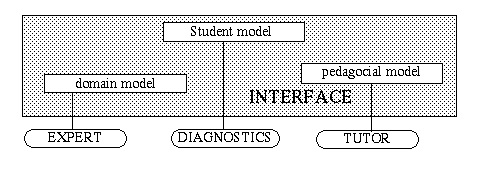
\includegraphics[]{img/ITS-components.jpg}
	\caption{Komponente ITS-a}
	\label{fig:its-comp}
\end{figure}

\subsubsection{Domenski model}
Domenski model je dio sustava čiji je smisao organizirati znanje u jedinice spremne za pohranu u bazu podataka. Svaki sustav osmišljava vlastitu podjelu znanja s obzirom na različitu širinu podjele i broj razina. U pravilu je neizbježna podjela na predmete u složenim sustavima i koncepte unutar predmeta, a na autorima i administatorima sustava je definirati više ili niže razine u odnosu na koncepte. Granulacija znanja je zato prilično kompliciran posao većoj količini autora, no budući da je kreiranje domenskog modela kreativan posao, u procesu zamišljanja treba sudjelovati što veći broj ljudi.
\par
Domenski model ne uključuje samo podjelu znanja, nego i pravila te strategije koje treba naučiti. Oni se mogu prikazati eksplicitno formulama i materijalima za učenje ili implicitno redoslijedom prikaza pitanja ili slično. Implicitno zadavanje pravila i strategija tipično je za formalne školske sustave zato što postoji određen redoslijed predavanja te nastavnici očekuju da učenici/studenti poznaju gradiva prethodnih predavanja. U sustavima za elektroničko učenje takav je pristup teže izvesti te se pravila i strategije najčešće zadaju eksplicitno u obliku najniže razine podjele u bazi podataka, iako korisnik uglavnom tu eksplicitnost ne vidi.
\par
Prilikom kreiranja domenskog modela važno je misliti na to da je takav model kvalitetna reprezentacija različitih vrsta znanja, da bude efikasan i razumljiv za kreiranje algoritama te da može odgovoriti na potrebe korisničkog modela.
\par
Tipični domenski model je kvalitetno organizirana baza podataka te pravilno uneseni podaci. Za sve iznad toga se brinu ostale komponente, počevši sa korisničkim modelom.

\subsubsection{Korisnički model}
Učenički, studentski ili jednostavno korisnički model je komponenta sustava čija se svrha većim dijelom preklapa s domenskom komponentom i modelom učenja. Razlog odvajanja korisničkog modela je bolja analiza znanja pojedinog korisnika. 
\par
Korisnički model su uglavnom algoritmi koji analiziraju točnost odgovora (te možda daju dodatne savjete korisniku) i algoritmi koji omogućuju prikaz analize odgovora korak po korak. Zbog relativno male opsežnosti, neki izvori zanemaruju korisnički model cijepajući njegove dijelove u domenski i model učenja.

\subsubsection{Model učenja}
Nakon postavljanja domenskog i korisničkog modela, ostatak aplikacijske logike sadržan je u modelu učenja. Upravo je model učenja najbitniji dio inteligentnog sustava za elektroničko učenje jer on zamjenjuje ljudskog učitelja. Ovoj komponenti pripadaju algoritmi koji na temelju rezultata prethodno navedenih evaluiraju znanje korisnika, algoritmi korisnikove navigacije sustavom te algoritmi posluživanja pitanja.
\par
Svrha modela učenja je praćenje korisnikova napretka u pojedinim konceptima/predmetima. Iako je na prvi pogled to relativno jednostavan problem, on jest takav za ljudskog učitelja, ali za računalo nije. Takvi problemi umjetne inteligencije (UI) nazivaju se UI-potpuni. Nakon što algoritmi procijene znanje korisnika, ono se treba prikazati nekim vizualnim načinom da korisnik bolje razumije što ne zna i zašto mu sustav postavlja neka pitanja.
\par
Model učenja je srž ITS-a te glavni odraz kvalitete pojedinog sustava. Čest način implementacije modela učenja je logičkim produkcijama koje dovode do zaključka je li korisnik nešto naučio ili ne. Prednost takvog pristupa je formalna evaluacija korisnika i sustava samog, no nedostatak mu je nejasnost širem spektru administratora. Alternativni način je sustav bodovanja pojedinih pitanja, skupova pitanja i odnosa između koncepata koje korisnik treba savladati.

\subsubsection{Korisničko sučelje}
Korisničko sučelja je standardan element gotovo svake računalne aplikacije. Ono nužno ne mora biti grafičko, iako je takvo sigurno zanimljivije kranjem korisniku. Učenik treba vidjeti svoj trenutni napredak prikazan na jasan način, razumjeti na koji način sustav komunicira s njim i on sa sustavom te područje koje pitanja ispituju.

\subsection{Karakteristike dobrih sustava}
Nakon definiranja komponenata sustava za inteligentno učenje, potrebno je razmotriti koje karakteristike imaju kvalitetni sustavi za inteligentno učenje. Većina su obvezni dijelovi ITS-a te ih je baš zato važno navesti.

\subsubsection{Razrađena podjela znanja}
Iako se ovo čini kao očekivan uvjet iz  opisa domenskog modela, važno ga je ponoviti i u ovom dijelu. Ispravna podjela znanja omogućuje lakše i kvalitetnije projektiranje algoritama procjene korisnika. Postoje dvije razine razrade podjele znanja: projektiranje sustava - odabir mogućih granula, povezanosti između njih i načina evaluacije znanja te projektiranje pitanja - punjenje sustava pitanjima i formulama za evaluaciju u skladu s dogovorenom podjelom.
\par
Granulacija podjele znanja je pitanje bez jednoznačnog odgovora, a s puno rizika. Ukoliko sustav ima premalo razina podjele, postoji rizik od nedovoljno dobrog praćenja korisnikova znanja, a sustav s previše razina podjele zahtijeva ogroman broj različitih pitanja da svaka od razina ima reprezentativni uzorak ocjene korisnika.
\par
Elegantno rješenje problema je određivanje srednje velikog broja granulacija (jasno, što je srednji broj ovisi o opsegu domene za koju se ITS projektira), a onda između pojedinih granula uspostaviti različiti broj odnosa. Na taj način sam i ja riješio problem u svojoj implementaciji.

\subsubsection{Parametrizirana pitanja}
Zamislite slučaj u kojem ITS služi za formalnu provjeru znanja na fakultetu čiji studenti imaju organizirane forume na kojima dijele zadatke. Nerealno je očekivati da može postojati više od 20 pitanja neke domene, a postoji preko 500 studenata u generaciji. Kako osigurati adekvatnost provjere? Odgovor je jednostavan: parametrizacijom pitanja.
\par
Parametriziranje pitanja je postupak kojim se numerička (moguće i na tekstualnim, ali teže) pitanja u ITS zapisuju u obliku formula za evaluaciju. Korisnicima se prikazuju njihove vlastite vrijednosti pojedinih parametara, a točnost odgovora evaluira se formulom. Takav pristup ne samo da omogućuje jedinstvene vrijednosti različitim korisnicima, nego i različite vrijednosti istim korisnicima. Ukoliko neki korisnik želi ili mora više puta rješavati pitanja nekog koncepta, mogu mu se servirati jedinstvene vrijednosti parametara svaki put kada otvara to pitanje. Jedan od načina ostvarivanja parametrizacije pitanja je spremanje formule kao odgovora te popisivanja vrijednosti parametara i njihovih ograničenja (npr. imaginarni dio broja mora biti != 0, apsolutna vrijednost mora biti > 0 i sl.).

\subsubsection{Praćenje tipkanja i reakcija lica korisnika}
Jedna od najvažnijih karakteristika dobrog učitelja je uočavanje učenikovih reakcija, čitanje fizičkih znakova te zaključivanje iz toga. Najveći nedostatak sustava za učenje, kao i svake druge vrste udaljenog učenja, je fizička udaljenost učenika i učitelja. Stoga, elektronički sustavi za učenje moraju naći drukčije načine praćenja reakcija korisnika.
\par
Dva najpoznatija načina su praćenje tipkanja i izraza lica. Rastom količine prostora na tvrdim diskovima i brzine računala, stvorila se mogućnost praćenja naizgled trivijalnih detalja kao što je obrazac tipkanja pojedine osobe. Neki izvori kažu da svaka osoba ima jedinstven obrazac tipkanja, baš kao otisak prsta. Zato bi bilo važno pratiti u kojim je situacijama korisnik ubrzan, o kojim pitanjima dulje razmišlja te je li mijenjao neki odgovor.
\par
Praćenje izraza lica također je postalo moguće rastom brzine računala, njihove procesorske i grafičke snage te razvojem računalnog vida kao područja računarstva. Ideja takvog pristupa je aproksimirati ljudskog učitelja, no to je vrlo složen i težak posao. Nedostatak takvog pristupa je što svaki korisnik mora imati neki oblik web kamere.
\par
Oba dijela su dio najnaprednijih sustava s velikim budžetima za izradu zato što ih je složeno implementirati. 

\subsubsection{Prilagođene reakcije}
Neizostavna komponenta sustava za inteligentno učenje su reakcije (engl. feedback) temeljene na znanju korisnika. Jasno je da računalne aplikacije ipak ne mogu biti jedinstvene kao ljudski učitelji. Svejedno, reakcije sustava moraju biti kvalitetne i prilagođene pojedinom korisniku da bi ITS imao smisla. Postižu se analizom odgovora korisnika i njegova načina odgovaranja (trajanjem računanja, brojem izmjena odgovora prije potvrde i sl.) te dobrim projektiranjem sustava (postojanjem reakcije za svaku kombinaciju razine znanja).
\par
Određivanje kada korisniku treba dati uputu (engl. hint) ako je zapeo na nekom zadatku je pitanje bez jednoznačnog odgovora, uostalom, kao i ljudskim učiteljima. S jedne strane učitelj mora znati detektirati kada je njegov učenik iscrpio sve mogućnosti, a s druge je jasno da otvoreno pitanje u sustavu za elektroničko učenje može značiti to da je korisnik jednostavno otišao od svojeg računala. Dva rješenja koja se nameću su pamćenje mogućih pogrešnih kombinacija parametara i broja pokušaja te dopuštanje korisniku da zatraži uputu ako sam shvaća da nema ideju. Nedostatak prvog rješenja je moguća prevelika nepotrebna složenost, a drugog to što umorni korisnici ponekad odustaju prerano.
\par
Alternativni način rješavanja reakcija je jednostavno pustiti korisnika da odgovori krivo i dati mu uputu nakon što završi provjeru.

\subsubsection{Sigurnost}
Sigurnost je jako važan element svakog sustava, a to se ističe u dva aspekta: zaštita osobnih podataka i sprječavanje lažnog predstavljanja. Iako osobni podaci u ITS-u gotovo sigurno ne bi trebali sadržavati osjetljive informacije, važno ih je zaštiti nekim sustavom lozinki.

\begin{figure}[htb]
	\centering
	
\includegraphics[]{img/security.jpg}
	\caption{Ilustracija oznake sigurne stranice}
	\label{fig:security}
\end{figure}

\par
Sprječavanje lažnog predstavljanja je puno zanimljiviji problem. Ukoliko sustav ima ugrađeno praćenje tipkanja korisnika ili izraza lica, prilično je očito da bi takav pristup minimizirao rizik lažnog predstavljanja. No, što ako nema? Alternativna opcija je formalno rješavanje ispita ITS-a uz prisustvo administratora što vodi do gotovo potpunog eliminiranja samostalnog učenja. Tako da niti to nije najbolje rješenje. Koje onda jest? Zapravo ga i nema, sustav nažalost mora vjerovati korisniku ako ne želi implementirati skupe tehnologije praćenja tipkanja ili računalnog vida.

\subsubsection{Kvalitetni algoritmi}
Kvalitetni algoritmi su nešto što se gotovo podrazumijeva ukoliko želimo kvalitetan sustav. Sljedeća lekcija govori više o algoritmima sustava za elektroničko učenje, no bilo ih je važno navesti i u ovoj.

\subsubsection{Dizajn sučelja}
Posljednja, ali ne i najmanje važna karakteristika ITS-a je dizajn grafičkog korisničkog sučelja. To nije važno samo za ITS, nego i za svaku drugu računalnu aplikaciju jer loše sučelje odbija korisnike više nego bilo što drugo. Prilično je teško definirati što je točno kvalitetno grafičko korisničko sučelje, no ono bi sigurno moralo imati sljedeće karakteristike: intuitivnost rasporeda kontrola, lakoća upravljanja (brzina, dosljednost, dozvole promjena kontrola), ugodan izgled (boje, fontovi, izbjegavanje neugodnih efekata promjena boja") te prikladan prikaz informacija.
\par
Korisničko sučelje ITS-a također bi se trebao držati nekih principa jedinstvenih za to područje. Tri najvažnija su: mogućnost traženja upute (također su opcije gumb za odustajanje ili ispis odgovora), konzistentnost znakovlja (npr. cos ili csin za kosinus, točka ili zarez kao decimalna oznaka) te prikaz napretka u pojedinoj granulaciji znanja.

\subsection{Algotimi sustava za inteligentno učenje}

\subsubsection{Odabir pitanja}
Vjerojatno najznačajniji algoritam sustava za inteligentno učenje je algoritam odabira pitanja. On može biti oblikovan na različite načine, no dva su najčešća: logičkim produkcijama koje nadopunjuju produkcije procjena korisnikova znanja ili samostalan programski odabir.

\subsubsection{Evaluacija odgovora}
\subsubsection{Procjena znanja}
\subsubsection{}

\subsection{Poznati sustavi}

\subsubsection{Neinteligentni sustavi}
Coursera? Doulingo? Računalne igrice (zbog AI, Dishonored)? Urban Jungle

\subsubsection{Inteligentni sustavi}

\subsection{Nedostaci ITS-a}

\subsubsection{Podučavanje i inteligencija}
Metode uspješnog podučavanja su očito najveći izazov svakog elektroničkog sustava za učenje. Iako neki izvori navode da kod problema koji se mogu rastaviti na sitne korake elektronički sustavi i ljudski učitelji imaju sličan rezultat usvojenosti gradiva kod učenika, podučavanje nije samo prenošenje znanja. Ono uključuje i metode usvajanja gradiva, procjene korisnikova znanja te oblikovanja odgovarajućih procesa učenja.
\par
Ponajveći problem metoda podučavanja i inteligencije ITS-a je što (zasad) nemaju pitanja "zašto?", "kako?" na korisnikov odgovor te kao takvi ne mogu dovoljno dobro procijeniti je li korisnik samo naučio "kuharicu", tj. formule za rješavanje zadataka. Jasno da sustav može pitati ta pitanja, no ona su svejedno organizirana po nekom predviđenom obrascu. Možda je nekada uputno pitati korisnika neka pitanja koja navodno zna kako bi bili sigurni da nešto stvarno razumije. Tu do izražaja dolazi intuicija učitelja koju sustavi (zasad) nemaju. Intuiciju donosi umjetna inteligencija temeljena na potpornom učenju, a ona je prilično različita od produkcijske umjetne inteligencije koju ITS koristi za definiranje je li korisnik nešto naučio.
\par
Drugi problem podučavanja je koliko korisniku sustav treba pomagati u rješavanju zadataka. Teza takve kritike je da korisnik jednostavno ne nauči dovoljno ukoliko mu sustav ponudi rješenje, da je takvo učenje previše površno. Osobno se slažem s tim pogledom i mislim da bi korisniku bilo korisnije prikazati bitnije upute tek nakon završene provjere, a onda ga manje kažnjavati (u dugoročnom pogledu) za krive odgovore.
\par
Naravno da je i problem ITS-a što autori pitanja jednostavno moraju odlično razumijevati tehničku pozadinu sustava (smisao pojedine granulacije, veze između granula) te ako ne razumiju ili sustav nije dovoljno dobro projektiran, u sustavu bi moglo doći do problema u definiranju korisnikova znanja ili otvaranju pitanja. Rizik površnog učenja je u takvim situacijama značajno veći.

\subsubsection{Cijena izrade}
Nadam se da je čitatelju jasno iz prethodnog dijela završnog rada da je izrada kvalitetnog ITS-a vrlo složen posao. Čak ne niti toliko težak, koliko opsežan. Problem izrade ITS-a je nužna bliska suradnja između računalnih stručnjaka i učitelja domene primjene. Velik broj ljudi koji moraju raditi istovremeno znači da je potreban velik broj radnih sati, što znači da ih treba platiti. Ukoliko vlasnik sustava ne očekuje da će mu ITS značajno povećati broj korisnika, logično je postaviti pitanje opravdanosti investicije. Pogotovo imajući u vidu cijenu održavanja sustava i rizik pogreške u sustavu. Zato je dosad ITS-ove uglavnom razvijala akademska zajednica.

\begin{figure}[htb]
	\centering
	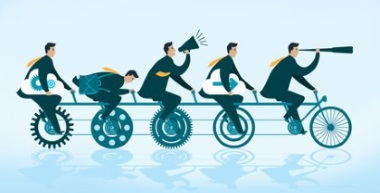
\includegraphics[]{img/teamwork.jpg}
	\caption{Ilustracija timskog rada potrebnog za dobar ITS}
	\label{fig:teamwork}
\end{figure}

\par
Drugi problem kod cijene izrade je kompleksnost sustava. Sustav za učenje jednostavno mora biti efikasan i brz, a sustav koji prati sve faktore to jednostavno ne može biti. Inženjeri koji ga projektiraju moraju napraviti \textit{trade-off} između brzine i kvalitete sustava.

\chapter{Slojevi aplikacija}
Sve kvalitetno oblikovane moderne aplikacije moraju sadržavati nekoliko slojeva rada. Slojevita arhitektura omogućuje sigurno zadržavanje dva najvažnija logička načela dobrog oblikovanja: nadogradnju bez promjene i načelo jedinstvene ovisnosti. Takav pristup također intervencije u kod aplikacije čini lakšim. Arhitektura koju koristim je MVC (Model - View - Controller). Prevedeno na hrvatski, model je podatkovni sloj, controller je aplikacijska logika, a view pogled. Najveća prednost ovakvog pristupa je jednostavna i intuitivna višeplatformska modularnost - podatkovni sloj je zajednički za sve platforme, aplikacijsku logiku može koristiti više različitih platformi (npr. kod pisan u Javi za Android i web aplikacije ili C\# za Windows 10 i web), a svaka platforma određuje svoje korisničko sučelje, tj. pogled.

\begin{figure}[htb]
	\centering
	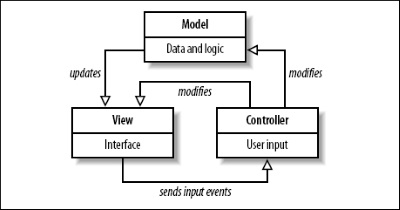
\includegraphics[]{img/mvc.jpg}
	\caption{Komunikacija u MVC modelu}
	\label{fig:mvc}
\end{figure}

\par
Podatkovni sloj je sloj pohrane, dohvata i ažuriranja podataka, gotovo uvijek izveden u obliku baze podataka te ponekad pripadnih tehnologija kao npr. Entity Framework koji mapira objekte i bazu podataka. Podaci spremljeni u podatkovnom sloju moraju biti u \textit{display-neutral} obliku, što znači da bez daljnje obrade nisu previše pogodni za sami prikaz. Cilj takvog pristupa spremanja podataka je imati bazu u prve tri normalne forme te posljedično očuvati performanse baze na visokoj razini čak i uz veću količinu podataka spremljenih u nju. Podatkovni sloj implementiran u ovom završnom radu je SQL baza podataka te Entity Framework.
\par
Aplikacijska logika je sloj upravljanja korisničkim zahtjevima, a radi kao poveznica između prikaza i podatkovnog sloja. Aplikacijska logika prima naredbe koje je korisnik zadao na pogledu, zatim provodi neke operacije nad modelom, uzima podatke iz modela te ih u \textit{display-neutral} obliku šalje pogledu. Ona je uglavnom implementirana kao nekoliko slojeva različitih poslova, npr. \textit{utlity} sloj rada s bazom, sloj koji prima podatke od pogleda te algoritamski sloj koji provodi operacije. U ovom završnom radu aplikacijska logika će upravo raditi na taj način: statičke klase rada s bazom, klase algoritama odabira pitanja te klase koje primaju pozive operacija s korisničkog sučelja.
\par
Pogled, tj. korisničko sučelje je način na koji se aplikacija prezentira kranjem korisniku te način na koji je on koristi. Njegov je cilj rada obraditi podatke tako da ih može lijepo i kvalitetno prikazati korisniku te slati zahtjeve korisnika aplikacijskoj logici. Budući da zadatak ovog ZR nije implementirati taj sloj aplikacije, jedino korisničko sučelje koje će se koristiti je ono za administratora koji mora moći dodavati nova pitanja, generirati testove i slično.
\par
Uspoređujući slojeve inteligentnog sustava za elektroničko učenje i MVC višeslojne aplikacije, vidimo jasnu povezanost izemđu domenskog modela i modela kao dio MVC-a, controllera te korisničkog modela i modela znanja te grafičkog sučelja i pogleda. Upravo to je smisao MVC pristupa, jednostavno je logičan za ogromnu količinu situacija. Zašto onda ovaj završni rad navodi oba? Zato što je MVC tehnološki presjek, a slojevi ITS-a logički. Njihovo poklapanje je potvrda da je aplikacija projektirana na ispravan način. Filozofskiji odgovor bi bio da je MVC pogled programskog inženjerstva na aplikaciju, a slojevi ITS-a računarske znanosti.

\chapter{Opis implementiranog rješenja}
Opis rješenja

\section{Korištene tehnologije}
SQL, C\#, Java, Entity Framework,
SQL Management Studio, Visual Studio, Eclipse, Android Studio

\section{ER dijagram}
ER

\section{Mogućnosti sustava}
mogućnosti

\subsection{Parametrizirana pitanja}

\subsection{baza stanja, stablo znanja, whatever}

\subsection{Mogućnosti administratora}

\subsection{Mogućnosti korisnika}

\section{Logika posluživanja pitanja}
logika

\chapter{Zaključak}
Zaključak.

\bibliography{literatura}
\bibliographystyle{fer}

\begin{sazetak}
Sažetak na hrvatskom jeziku.

\kljucnerijeci{Ključne riječi, odvojene zarezima.}
\end{sazetak}

% TODO: Navedite naslov na engleskom jeziku.
\engtitle{Application logic and data layer development for an e-learning system}
\begin{abstract}
Abstract.

\keywords{Keywords.}
\end{abstract}

\end{document}
